\chapter{Bąkiem malowane}
\markboth{Bąkiem malowane}{Bąkiem malowane}

Ponieważ niektóre otrzymywane ślady ruchu bąków bywały niezwykle artystyczne i wprawiały nas w zdumienie zdecydowaliśmy się pokazać co ciekawsze ku uciesze czytelnika. Zestaw śladów, który najbardziej przypadł nam do gustu przedstawiono na rysunku \ref{fig:top_life} \cite{Joniak}.
\begin{figure}[tp]
  \centering
  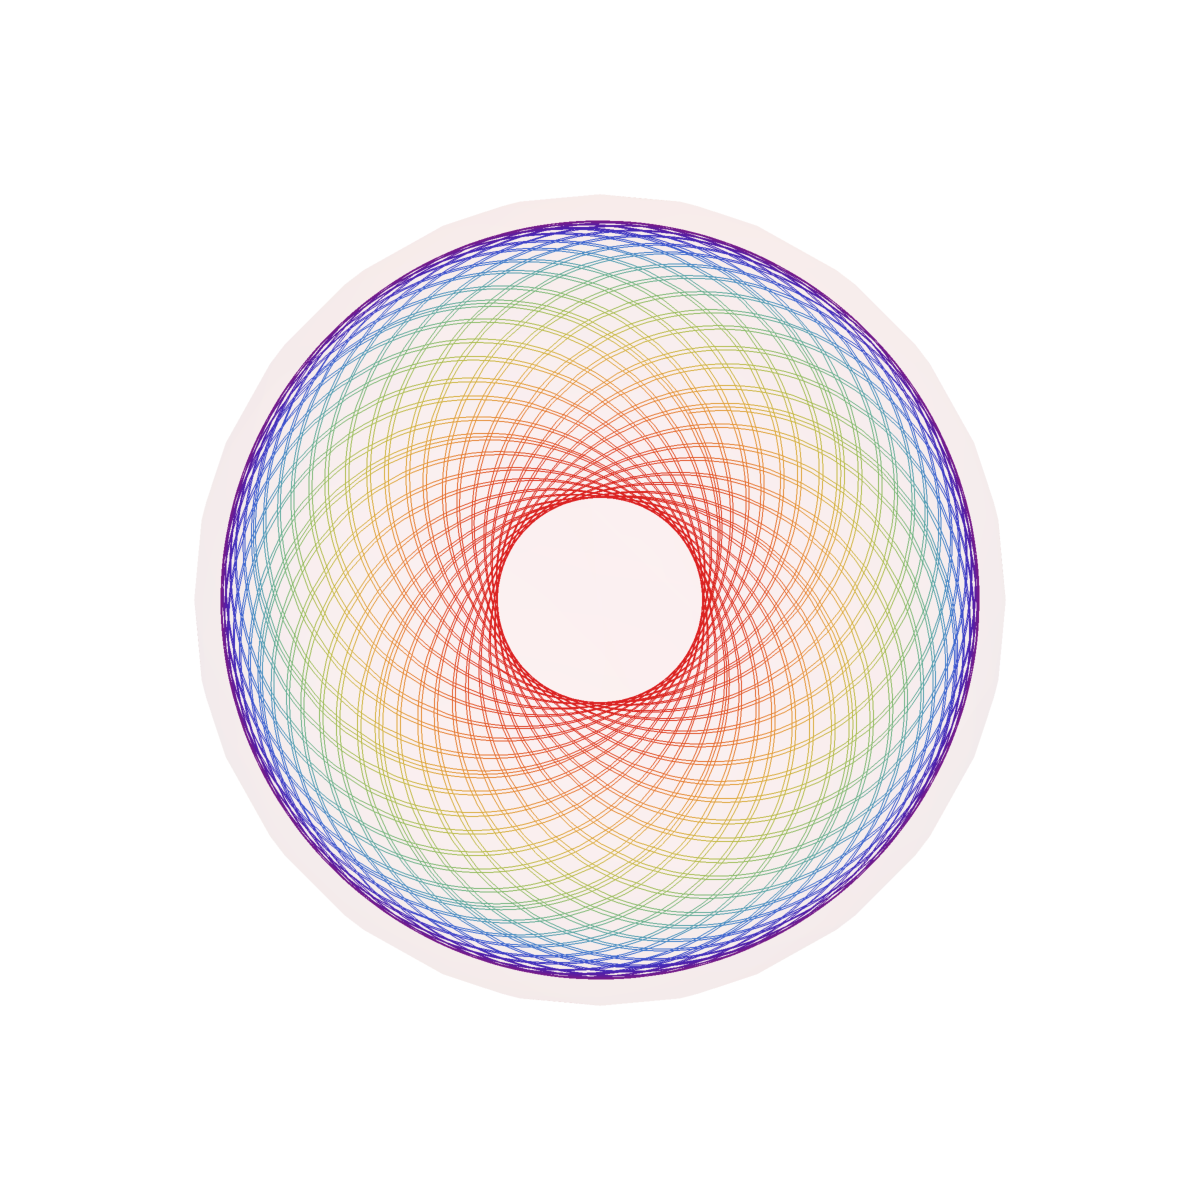
\includegraphics[scale=0.7]{figures/chapter_06/mal2.pdf}
  \caption{Atom}
\end{figure}
%
\begin{figure}[tp]
  \centering
  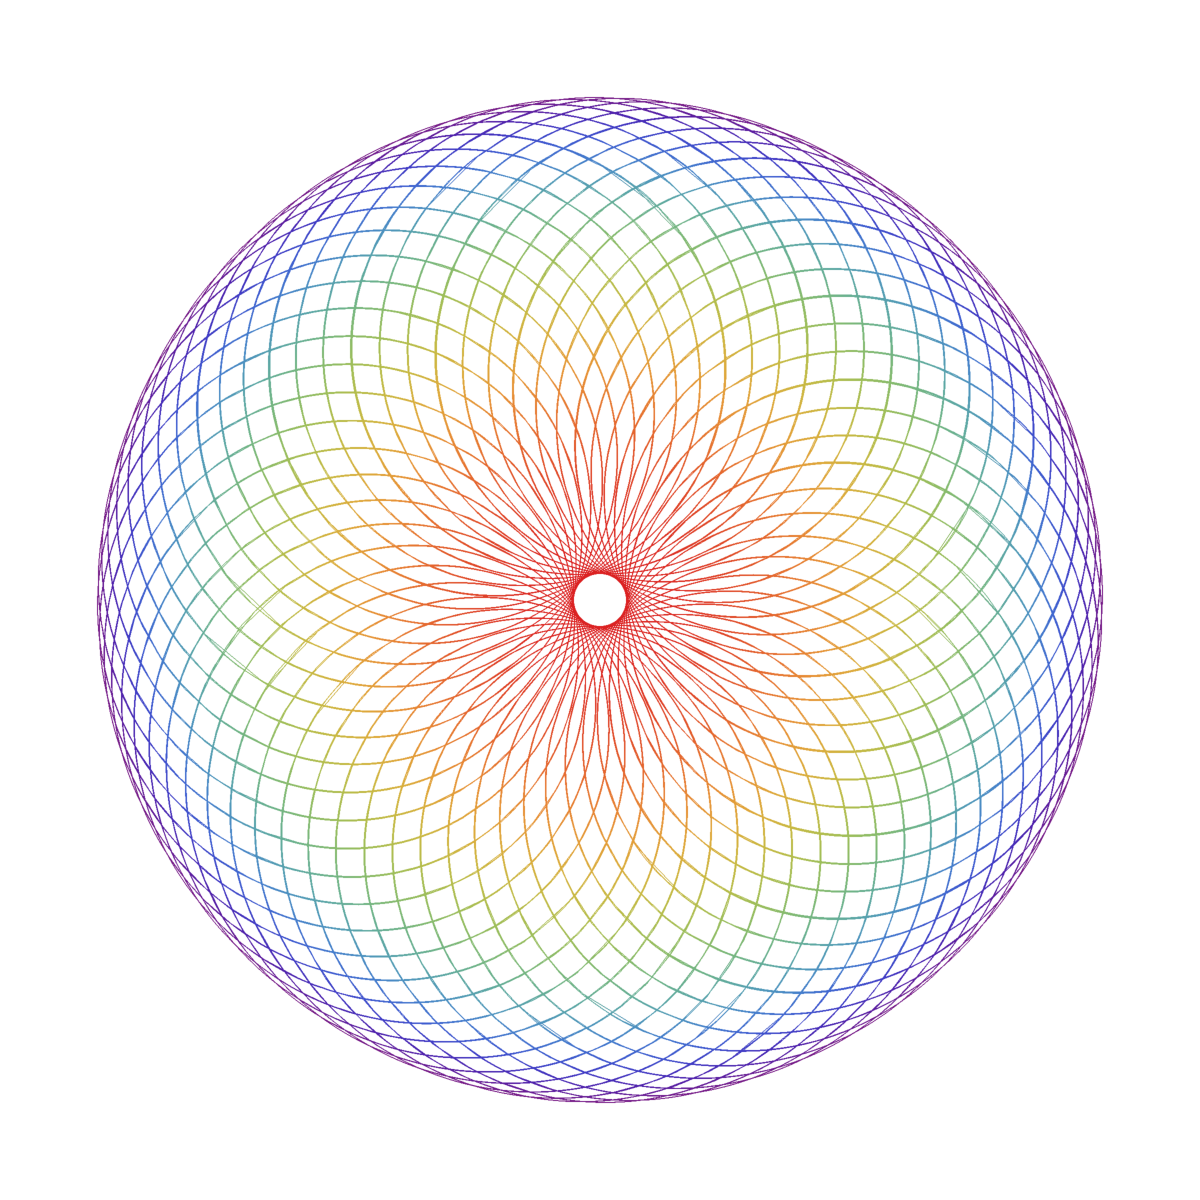
\includegraphics[scale=0.5]{figures/chapter_06/mal4.pdf}
  \caption{Słonecznik}
\end{figure}
%
\begin{figure}[tp]
  \centering
  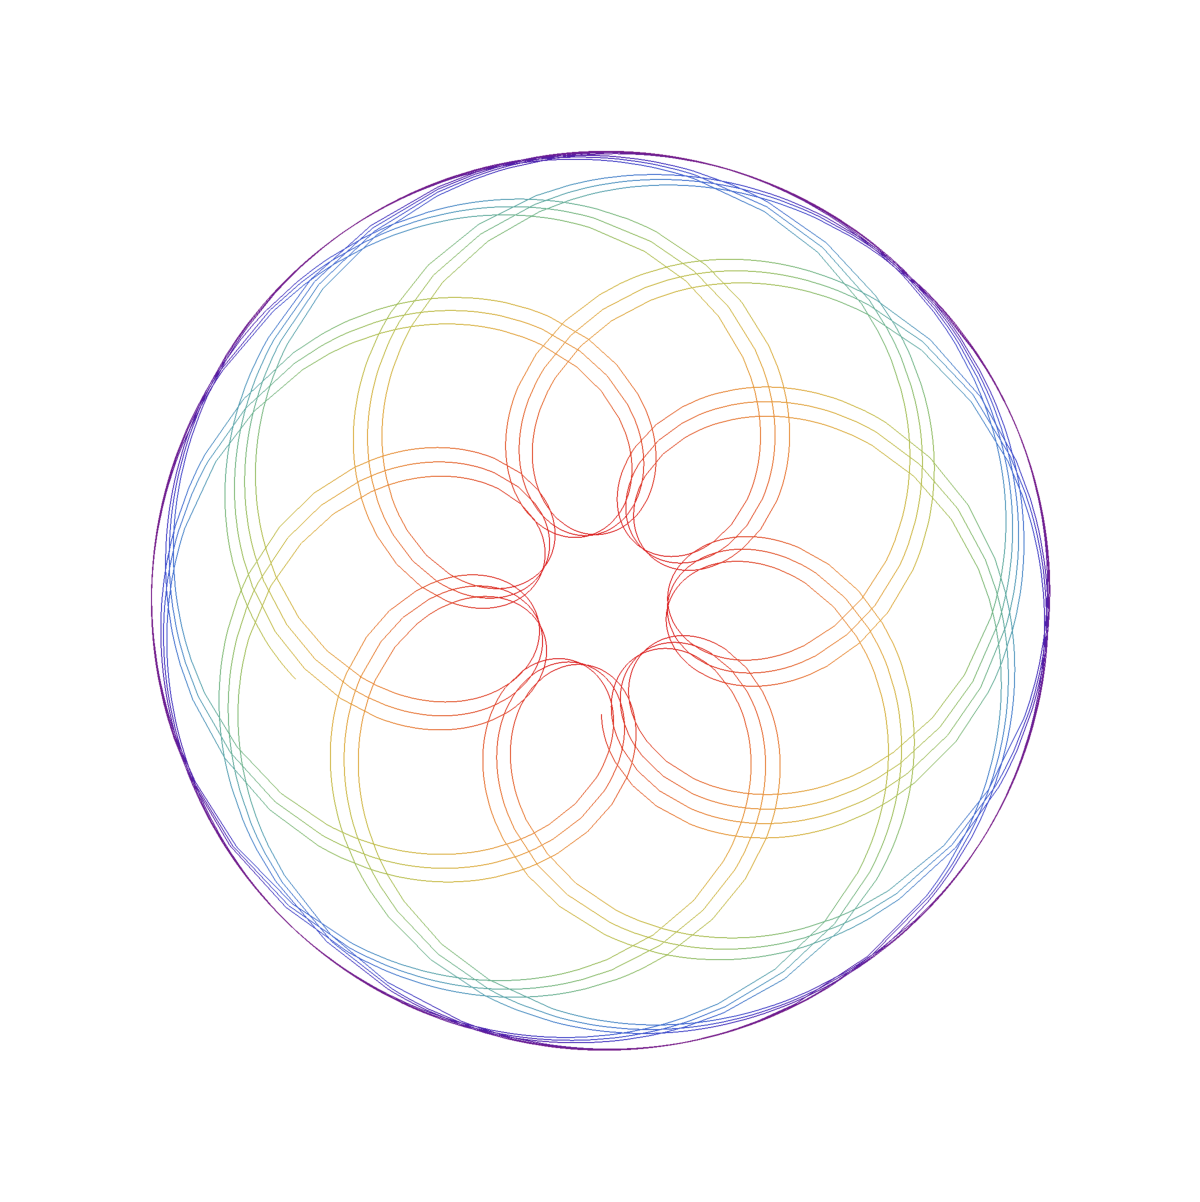
\includegraphics[scale=0.5]{figures/chapter_06/mal5.pdf}
  \caption{Kwiat}
\end{figure}
%
\begin{figure}[tp]
  \centering
  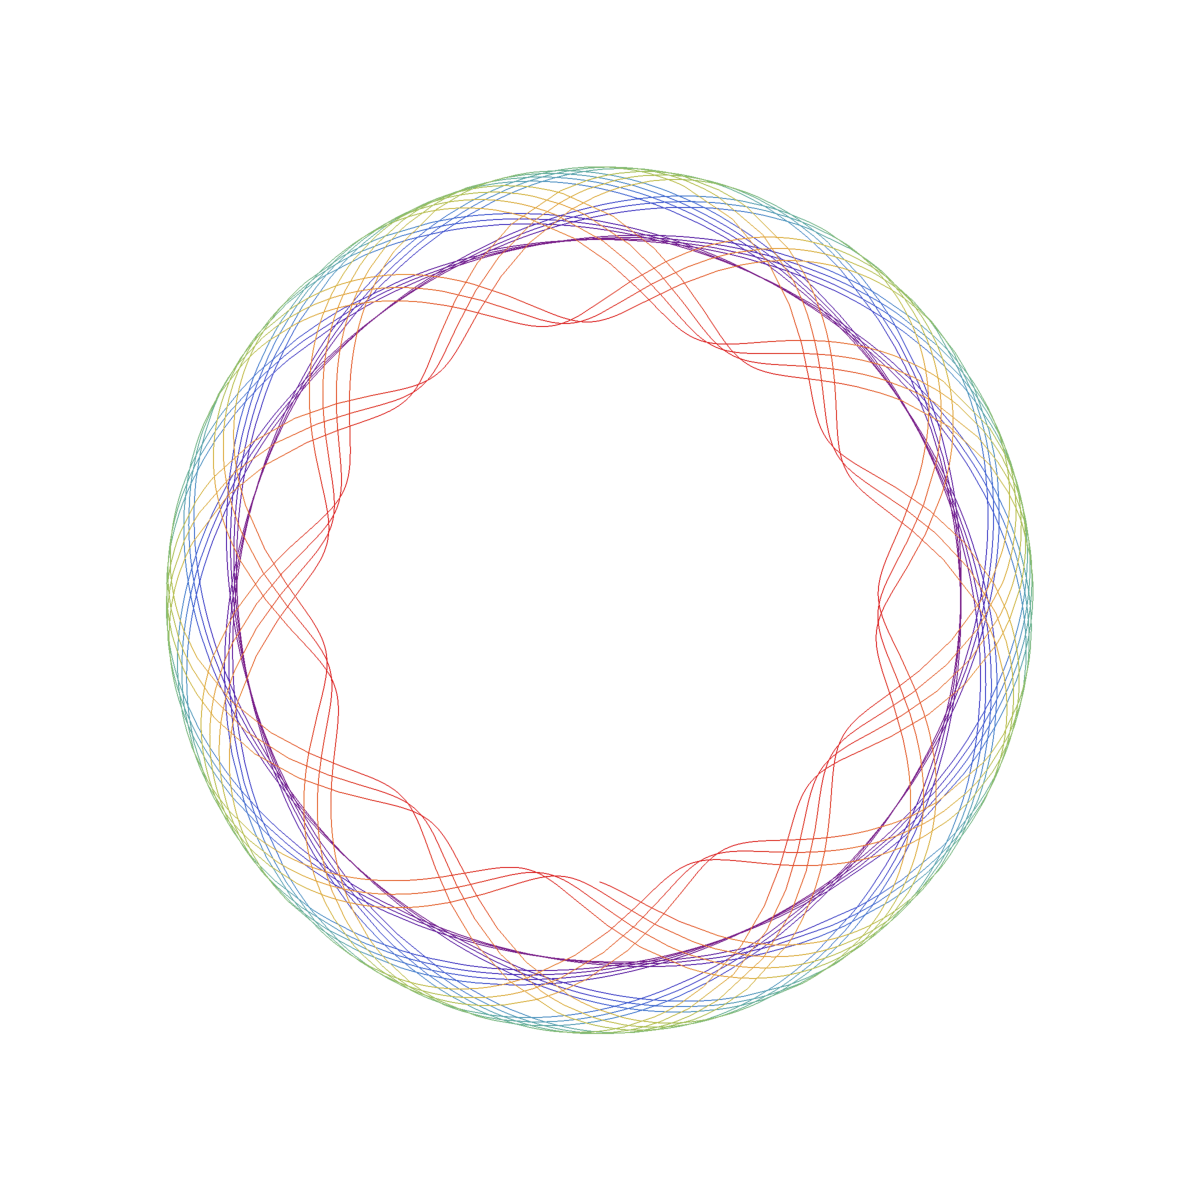
\includegraphics[scale=0.5]{figures/chapter_06/mal8.pdf}
  \caption{Gwiazda}
\end{figure}
%
\begin{figure}[tp]
  \centering
  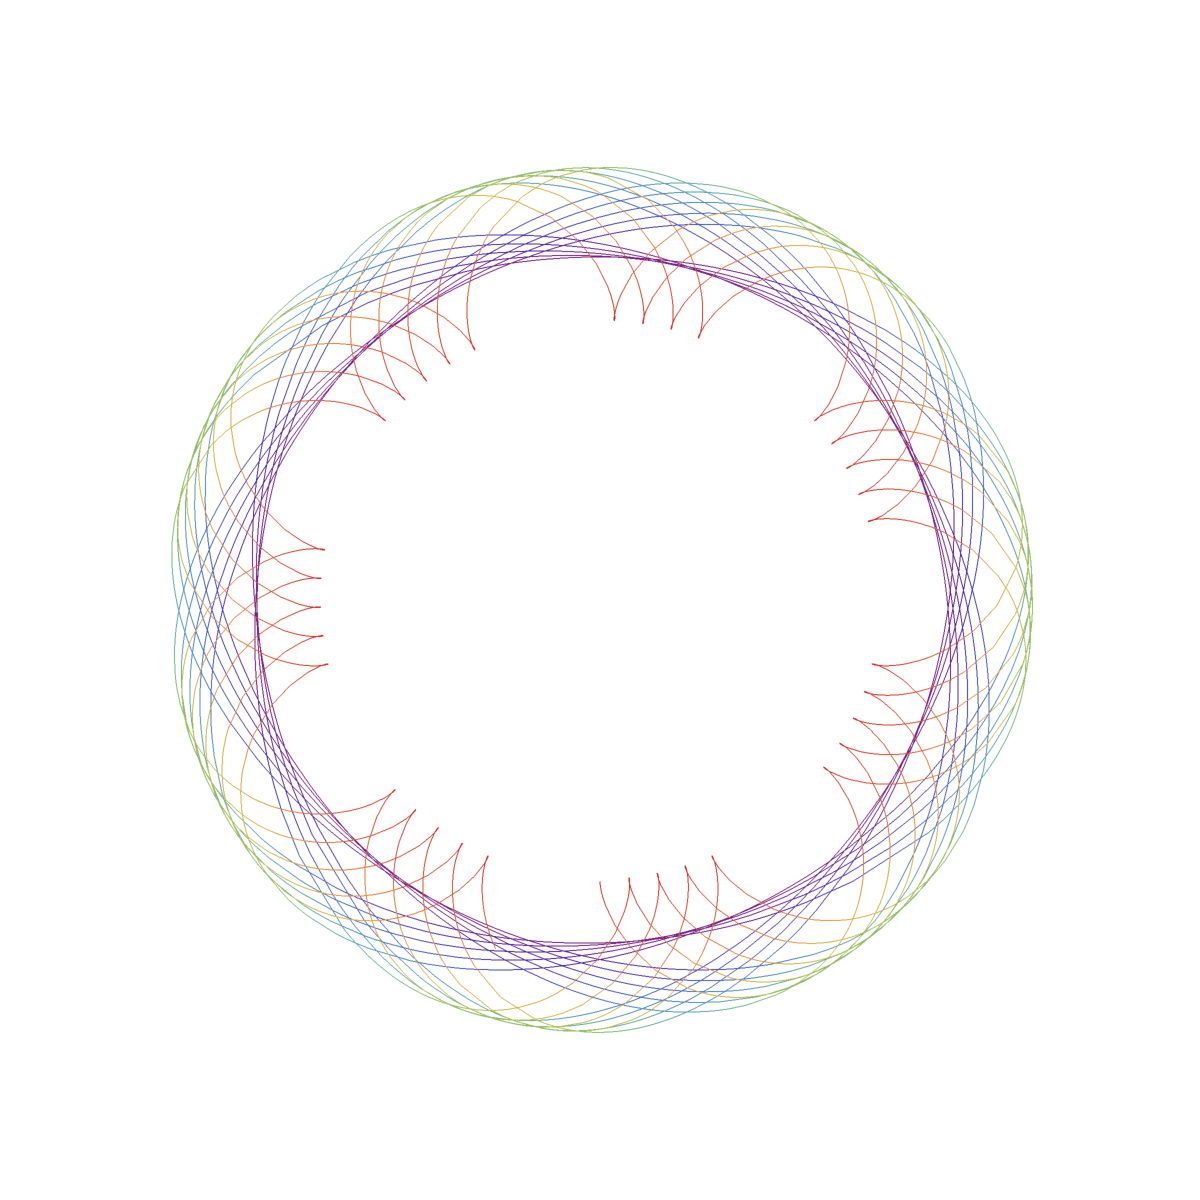
\includegraphics[scale=0.5]{figures/chapter_06/mal7b.pdf}
  \caption{Paszcza}
\end{figure}
%
\begin{figure}[tp]
  \centering
  \subfloat{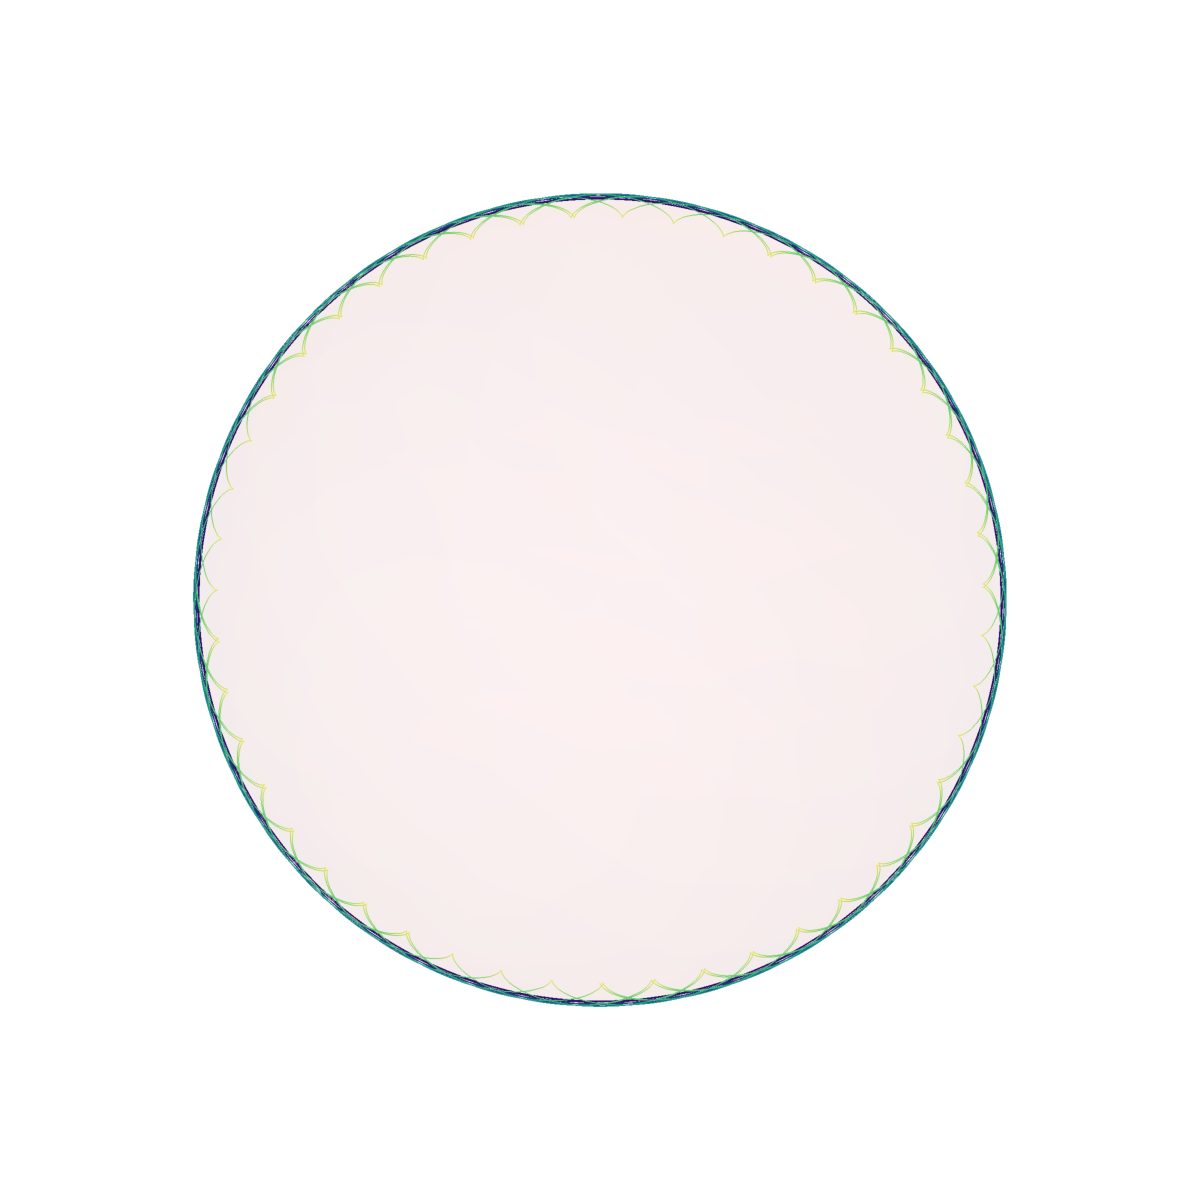
\includegraphics[scale=0.45,trim={2cm 2cm 2cm 2cm}, clip]{figures/chapter_06/malowane_-1.pdf}}
  \subfloat{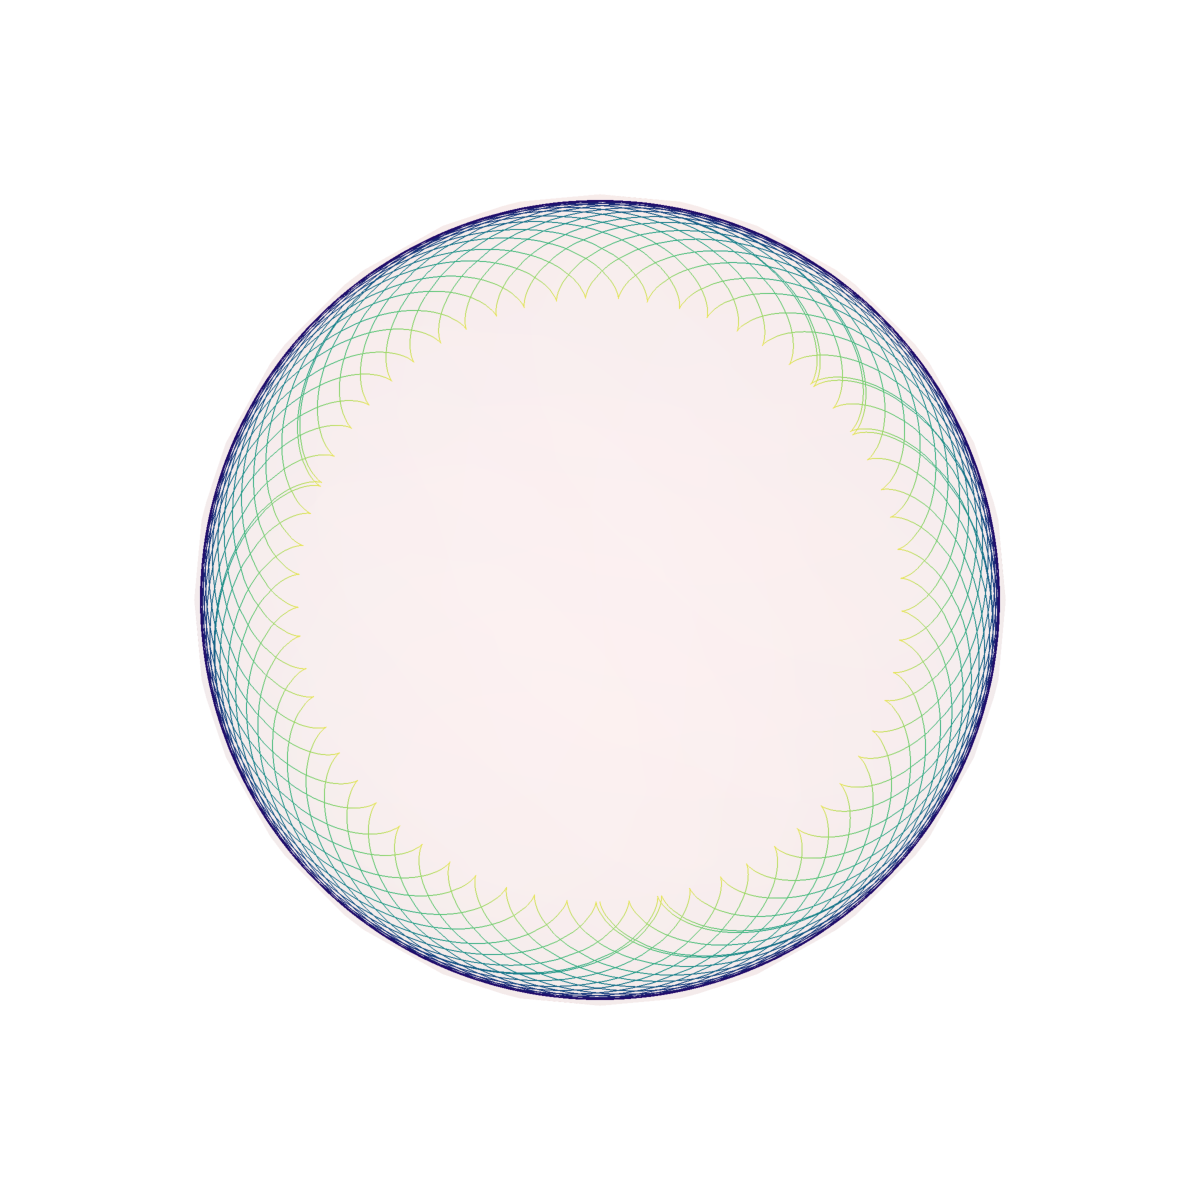
\includegraphics[scale=0.45,trim={2cm 2cm 2cm 2cm}, clip]{figures/chapter_06/malowane_4.pdf}}\\
  \subfloat{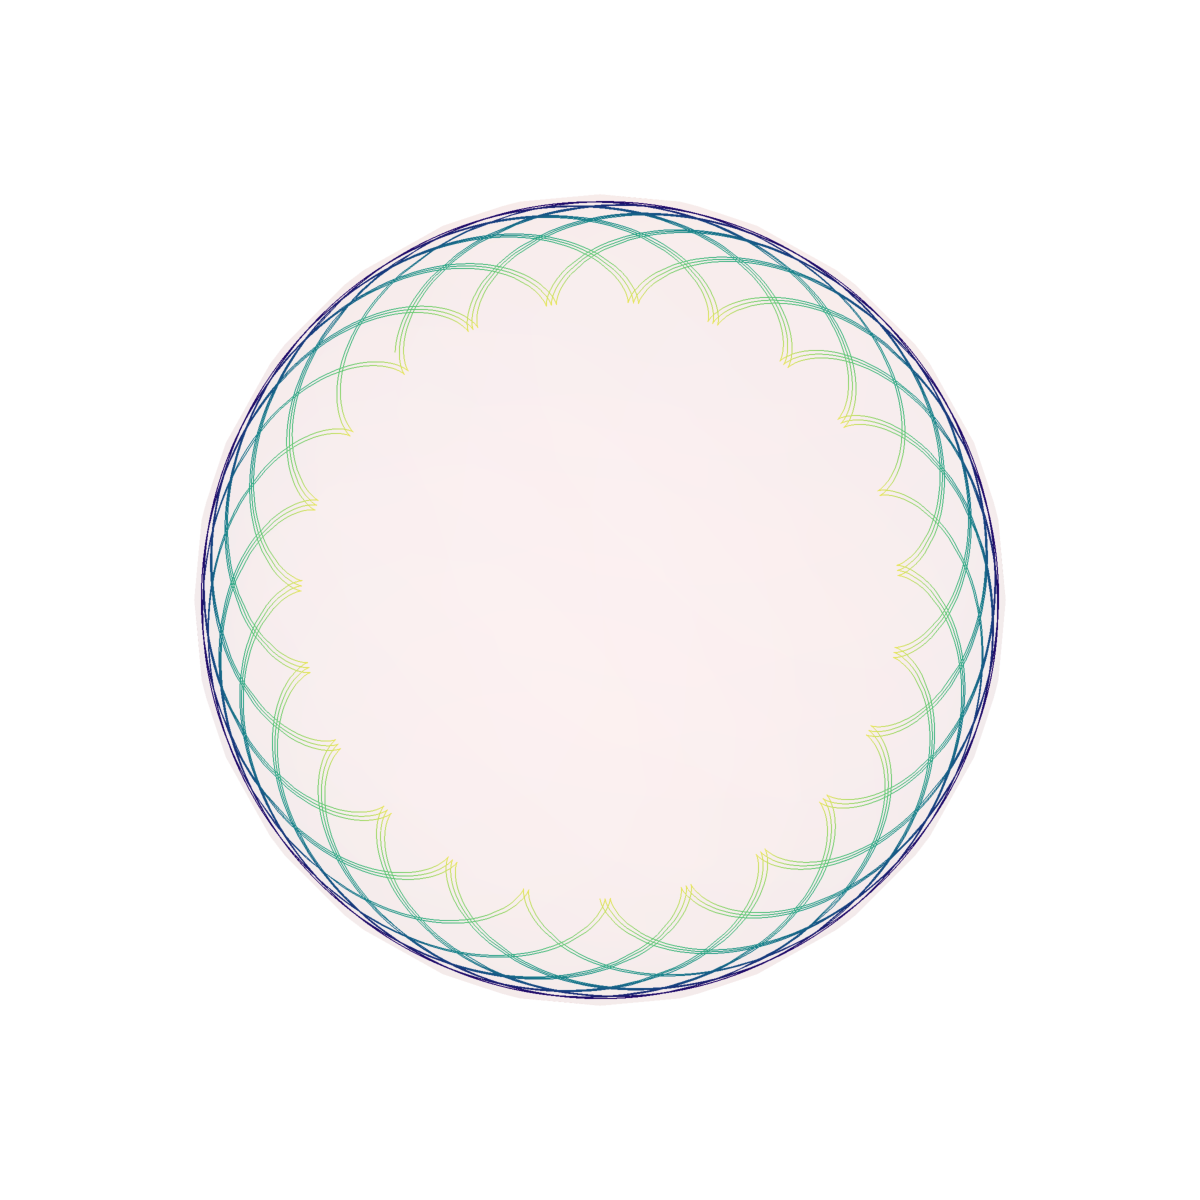
\includegraphics[scale=0.45,trim={2cm 2cm 2cm 2cm}, clip]{figures/chapter_06/malowane_0.pdf}}
  \subfloat{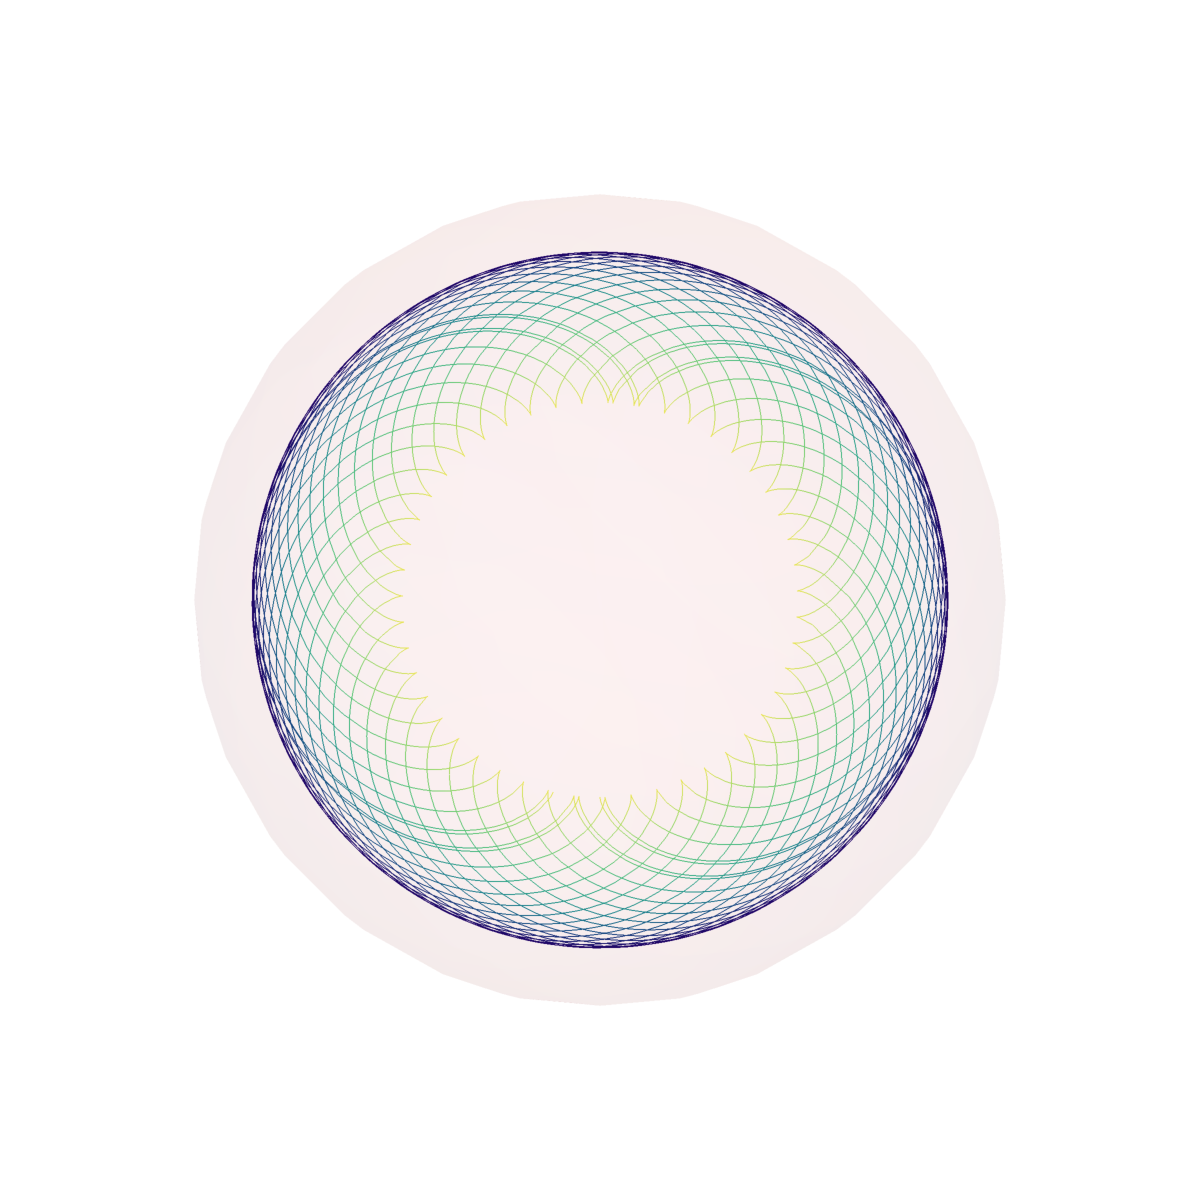
\includegraphics[scale=0.45,trim={2cm 2cm 2cm 2cm}, clip]{figures/chapter_06/malowane_2.pdf}}\\
  \subfloat{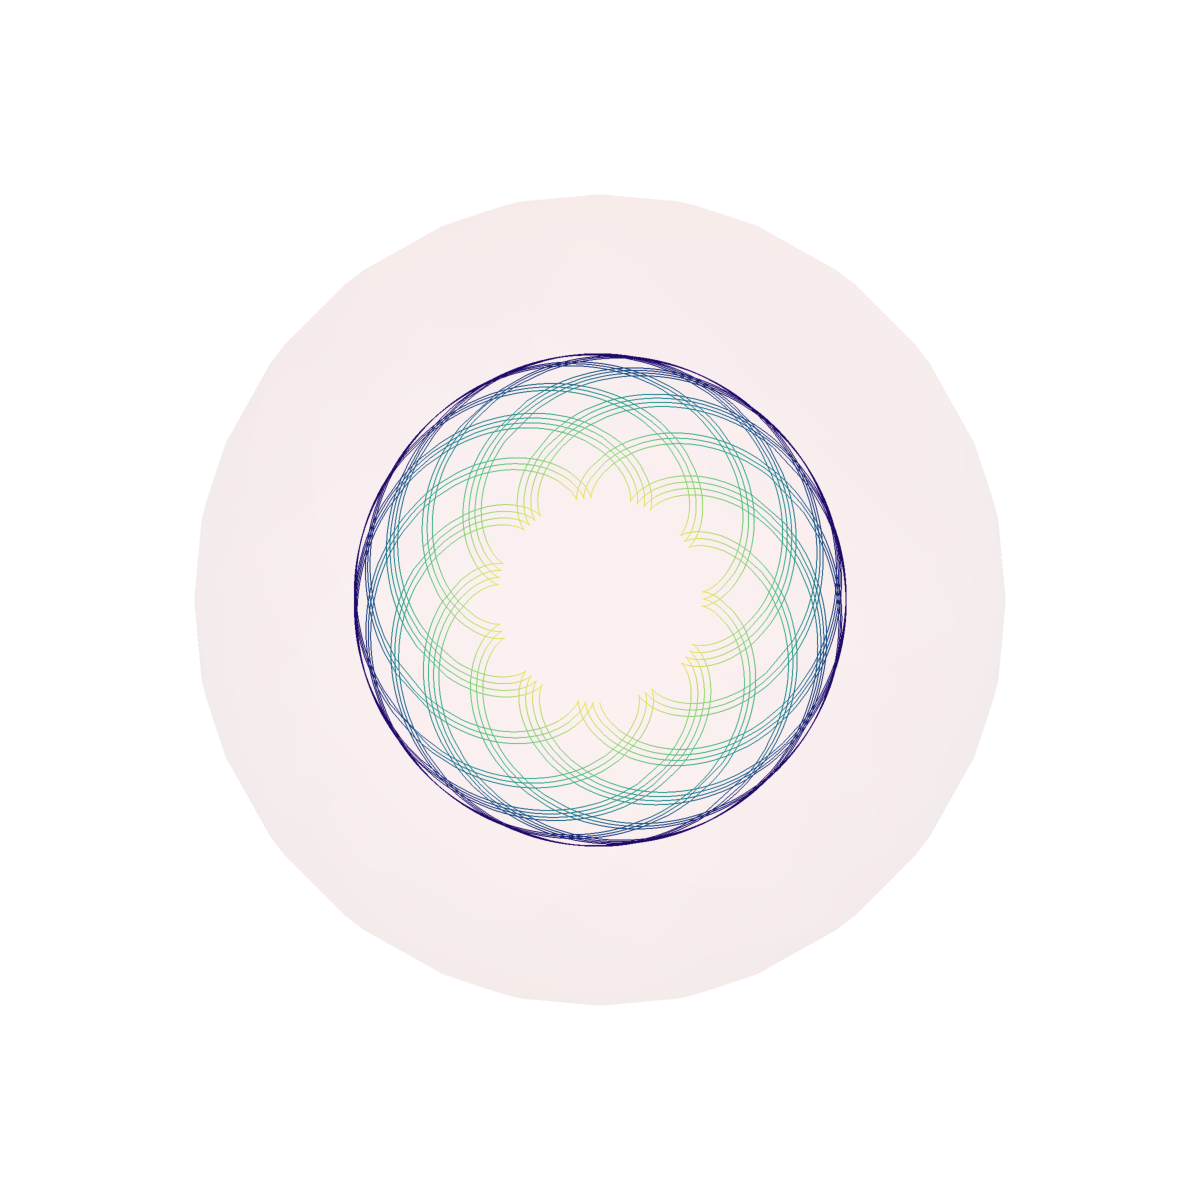
\includegraphics[scale=0.45,trim={2cm 2cm 2cm 2cm}, clip]{figures/chapter_06/malowane_3.pdf}}
  \subfloat{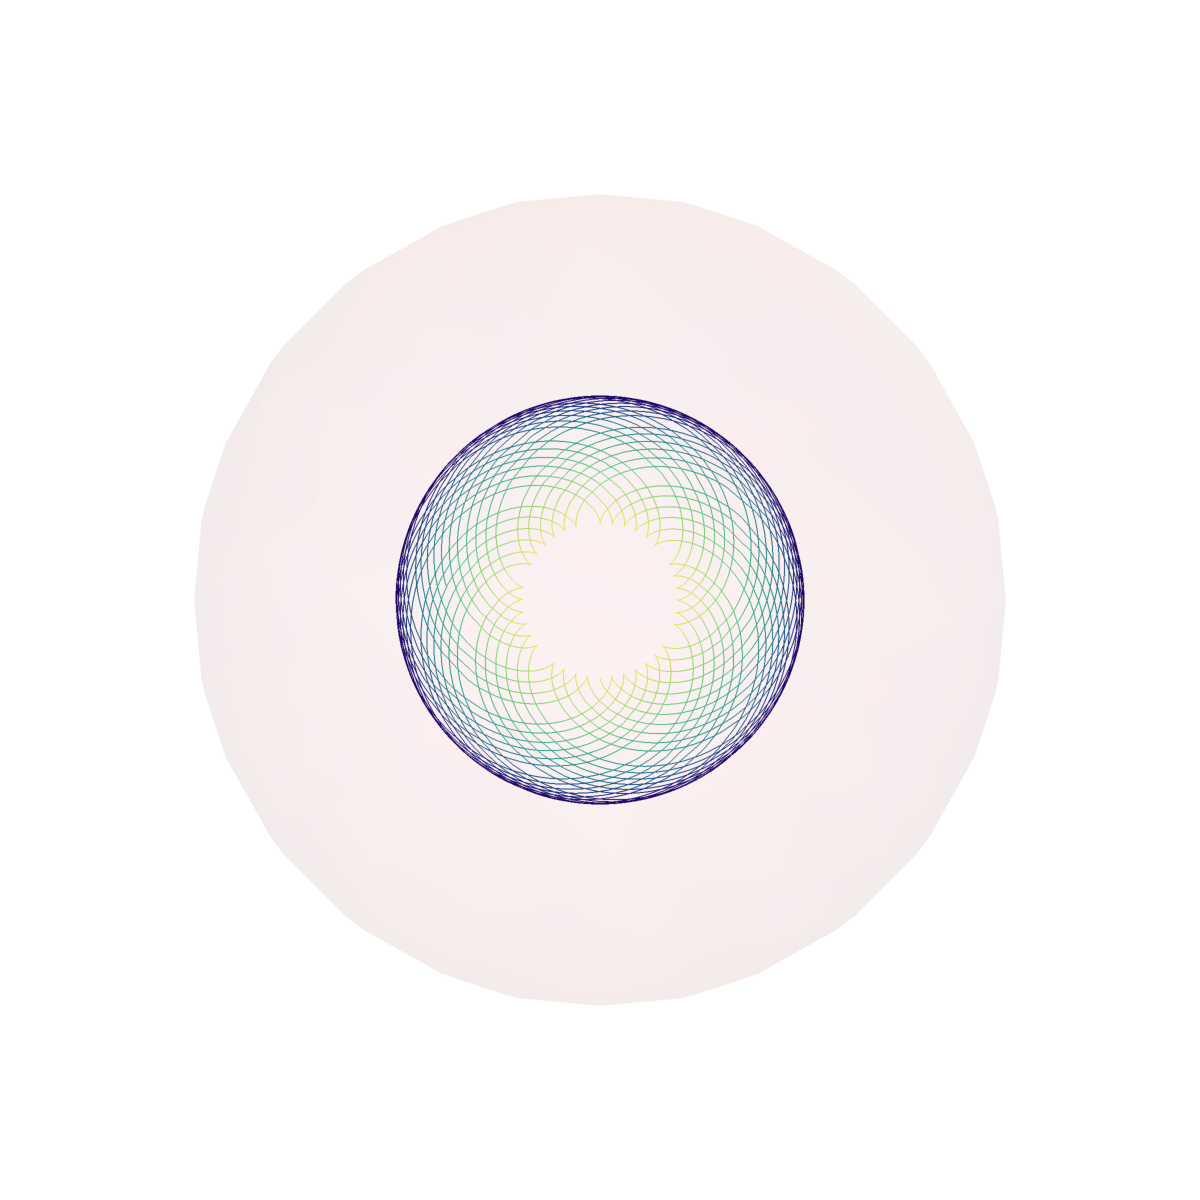
\includegraphics[scale=0.45,trim={2cm 2cm 2cm 2cm}, clip]{figures/chapter_06/malowane_6.pdf}}
  \caption{Życie bąka}
  \label{fig:top_life}
\end{figure}

{\red
  Czasami pojawia się potrzeba umieszczenia w~pracy dodatków. Wówczas
  wystarczy poprzedzić je poleceniem \texttt{\textbackslash appendix}
  i~voilà, mamy co potrzebowaliśmy. Tu można umieszczać rzeczy
  poboczne, kod programu, dowód jakiegoś twierdzenia, w~większej
  liczbie symulacje, wyniki, czy też może jakąś galerię \smiley}
